\section{Results}\label{sec:results}

\subsection{Variance decomposition}\label{sec:results-vc}

On the M3a-common analysis sample ($N=165{,}969$, 30 countries), the
empty model (M0) yields an L3 country ICC of $\rho_3=0.243$, an L2
country-year VPC of $\rho_2=0.025$, and an L1 share of $0.732$. The
L3 share sits inside the $0.15$--$0.25$ range reported by
\citet{SchmidtCatranFairbrother2016} for European trust outcomes;
the L2 share, while modest, is above the soft floor below which
a within--between decomposition adds little to a pure country-FE
specification. The decomposition therefore supports the three-level
specification.

Adding L1 controls (M1) reduces L1 residual variance by $5\%$ and
L2 country-year variance by $17\%$, while the L3 ICC drops marginally
to $0.241$. Adding L2 macro covariates and round dummies (M2) brings
the cumulative L2 variance reduction to $61\%$ and L3 to $13\%$:
the round dummies in particular absorb the global upward trend in
trust between R6 and R11, leaving the L2 VPC at $0.011$ (cf.\ M0's
$0.025$). The contrast between M3a (with round dummies) and M3b
(without) in Section~\ref{sec:results-headline} is designed to
surface the interpretive trade-off this absorption introduces.

Figure~\ref{fig:variance} visualises the variance decomposition
across the M0$\to$M6 progression as a stacked bar. The L3 share
contracts as covariates that are correlated with country differences
are added, and the random slope in M4 absorbs further L3 variance
into a slope variance not displayed in this projection.

\begin{figure}[!h]
  \centering
  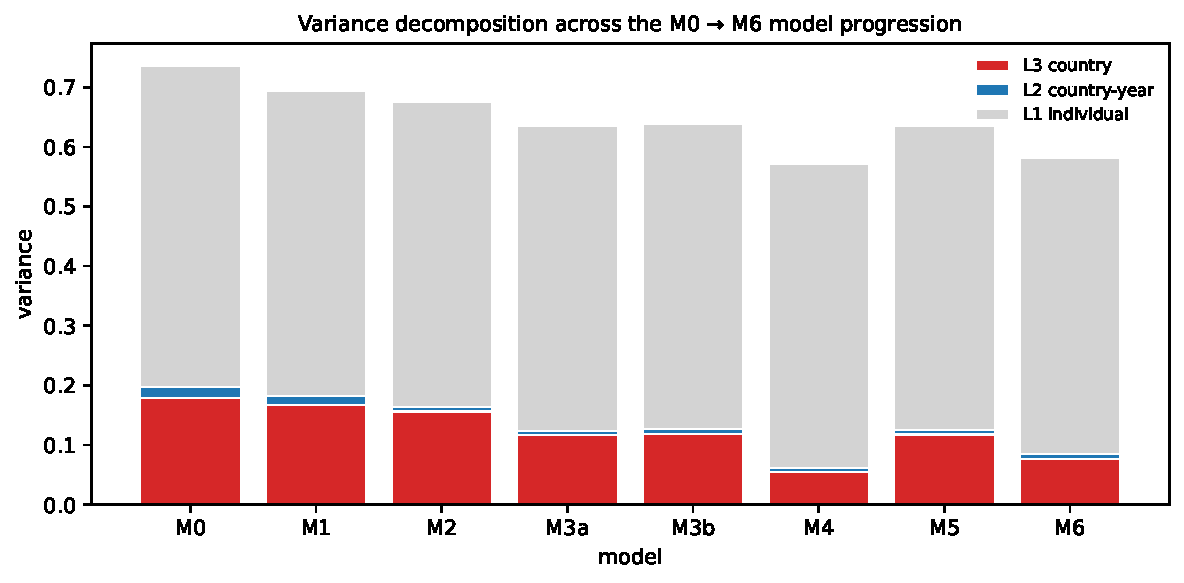
\includegraphics[width=0.85\linewidth]{figures/fig4_variance_components.pdf}
  \caption{Variance decomposition across the M0$\to$M6 model
  progression. L3 country variance contracts as country-correlated
  covariates and the random slope are added.}
  \label{fig:variance}
\end{figure}

\subsection{The within--between headline}\label{sec:results-headline}

Table~\ref{tab:models} reports the full M0$\to$M6 progression.
The Mundlak decomposition (M3a) is the substantive heart of the
analysis. The point estimates are
\[
  \hat\gamma_W = +0.024 \;(\mathrm{SE}\;1.123), \quad
  \hat\gamma_B = +11.239 \;(\mathrm{SE}\;3.427),
\]
with a Wald test of equality of $\chi^2(1)=9.66$, $p=0.002$. The
within-country effect is statistically indistinguishable from zero,
while the between-country effect is large, positive, and
significant. The cross-sectional positive correlation between AI
exposure and trust does not carry through to within-country
exposure shifts.

The sign of $\hat\gamma_B$ is the opposite of H1. Countries with
higher mean GenAI exposure---which are typically wealthier, more
service-economy-intensive, and have higher baseline institutional
quality---report \emph{higher} trust, not lower. This is the
selection / institutional-adaptation reading: the cross-sectional
correlation is confounded by everything that makes a country a
high-AI-exposure country in the first place. The M3b row, in which
$\hat\gamma_W = +1.46$ when round dummies are removed, attributes
to within-country exposure changes the global trend in trust over
2012--2024 that round dummies otherwise absorb; it is reported
alongside M3a precisely because the gap between the two clarifies
that the within-country exposure shifts identifiable separately
from the time trend are not detectably correlated with trust.

Figure~\ref{fig:caterpillar} shows the country random intercepts
(BLUPs) from M3a. Cross-country heterogeneity in trust persists
after the L1, L2, and Mundlak controls: Northern European countries
(Denmark, Norway, Sweden, Finland, Iceland, Switzerland, the
Netherlands) cluster in the positive tail, while Eastern and
Southern European countries (Bulgaria, Hungary, Greece) cluster in
the negative tail. The M3a sample includes 30 of the 36 ESS
countries; six are dropped via macro listwise deletion: Israel and
Russia are not in Eurostat at all, while Albania, Ukraine, and
Kosovo lack the harmonised unemployment and HICP series, and the
United Kingdom has no UK observations in Eurostat's annual
unemployment dataset for the ESS panel period (a Brexit-era data
gap discussed in Section~\ref{sec:data}).

\paragraph{H3 (individual exposure).}
The individual-level GenAI exposure coefficient
$\hat\beta_{\mathrm{genai}}$ is small, positive, and statistically
significant in M1 onward ($+0.015$, SE $0.002$). H3 predicted a
\emph{negative} sign (the structural-grievance / loser-theory
prediction); the data return the opposite. The composition channel
through which individuals in AI-exposed occupations would
\textit{themselves} report lower trust does not run as the
single-country robot-exposure literature would predict. This sign
reversal is small in magnitude---a fraction of a hundredth of a
standard deviation per unit of standardised exposure---but
substantively complements the within-between gap: the cross-sectional
positive correlation between AI exposure and trust is structural
(driven by what makes a country a high-exposure country) rather than
experiential (running through individuals' direct exposure).

\begin{figure}[!h]
  \centering
  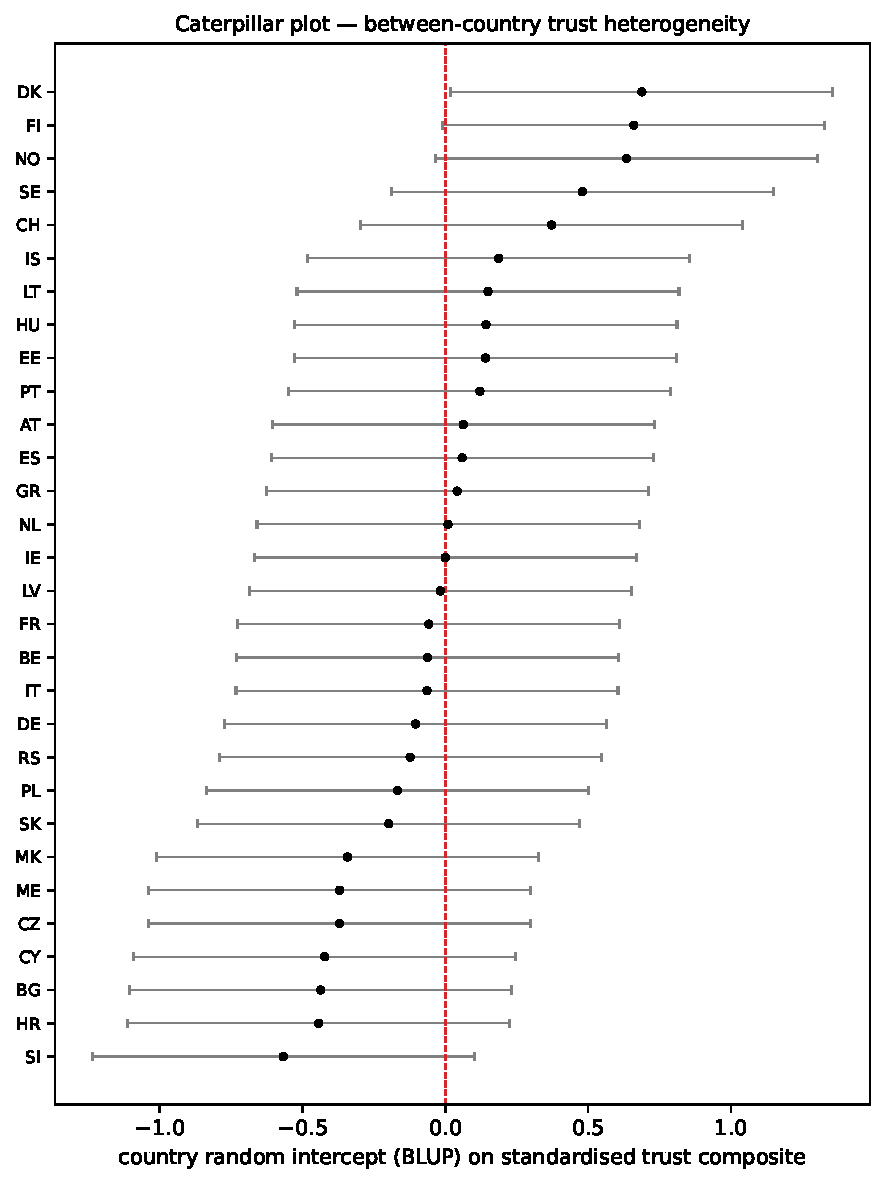
\includegraphics[width=0.55\linewidth]{figures/fig2_caterpillar.pdf}
  \caption{Caterpillar of country random intercepts from M3a
  (standardised trust composite). Error bars are
  $\pm 1.96\,\hat\sigma_{u_0}$ envelopes; cluster-specific
  posterior SEs are not exposed by \texttt{statsmodels.MixedLM}.}
  \label{fig:caterpillar}
\end{figure}

\subsection{Cross-level interaction (H4)}

M5 adds the within-exposure $\times$ education interaction. The
estimated interaction coefficient is $-0.142$ ($\mathrm{SE}\;0.130$,
$p=0.275$), a precise null. Neither H4a (substitution) nor H4b
(curator) is supported; the data prefer H4$_0$. The within-country
exposure effect, such as it is, does not vary detectably with
individual education. Figure~\ref{fig:interaction} plots the
predicted effect at each ISCED level over a plausible range of
within-country exposure deviations; the lines are visually
parallel, consistent with the null interaction.

\begin{figure}[!h]
  \centering
  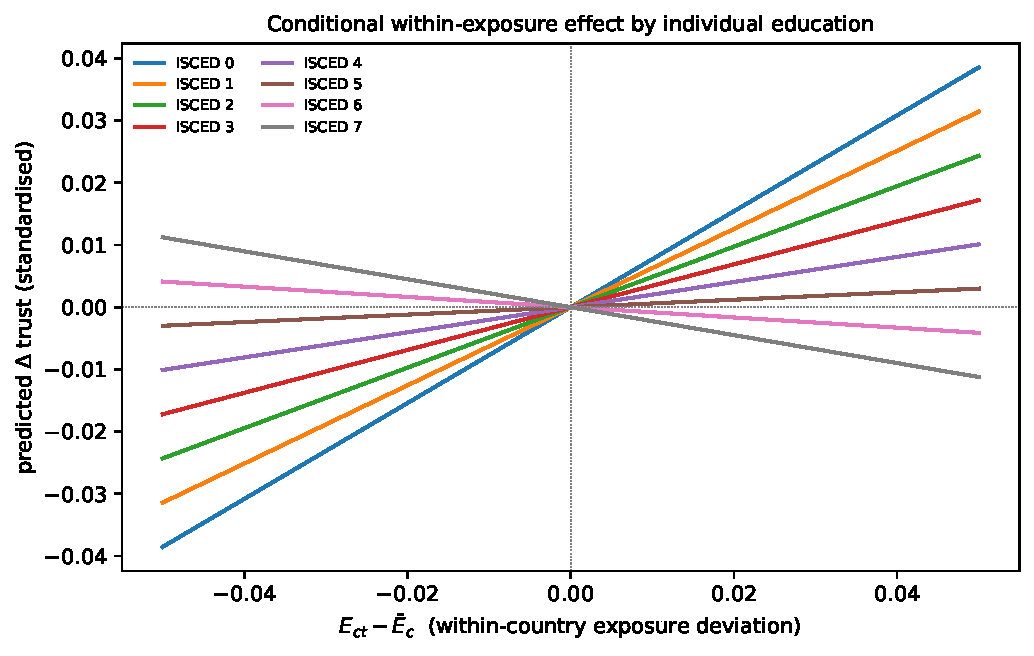
\includegraphics[width=0.85\linewidth]{figures/fig3_conditional_within_x_education.pdf}
  \caption{Conditional within-country exposure effect on trust by
  ISCED education level (M5). Lines are nearly parallel: the
  cross-level interaction coefficient is statistically zero.}
  \label{fig:interaction}
\end{figure}

\subsection{Institutional moderation (H5)}

The OECD EPL\,v1 (2007) baseline covers 23 of the ESS countries
(GB, IE, and the 21 continental, Nordic, Mediterranean, and
Eastern-European OECD members listed in Table~\ref{tab:descriptives}
notes); GB drops in M6 via the macro listwise deletion described
above, leaving 22 L3 units in the fitted sample. The within $\times$
EPL interaction is positive in sign ($+1.64$) but imprecisely
estimated ($\mathrm{SE}\;1.44$, $p\approx 0.26$). With only 22 L3
units, identification of an L3 moderator is intrinsically limited;
H5 cannot be rejected nor supported.

\paragraph{Note on the M6 education interaction.}
On the OECD subsample, the within $\times$ ISCED interaction
flips from the M5 null ($-0.142$, $p=0.275$) to a small but
nominally significant negative ($-0.318$, $\mathrm{SE}\;0.141$,
$p\approx 0.024$). The H4 conclusion is based on M5 because
(a) the larger sample is identified on the full European panel,
not the OECD-only subset; and (b) the M6 sample is selected on
non-missing EPL\,v1, which correlates with regime type and labour
market structure---making the M6 interaction a within-OECD
finding that may not generalise. We report it for completeness
in Table~\ref{tab:models} but treat M5 as the primary H4 test.

\begin{table}
\centering
\caption{Three-level multilevel models of the institutional-trust composite, M0--M6. Coefficients (standard errors). $^{*}\,p<0.05$. M5 is the primary H4 test on the full panel; M6 restricts to OECD ESS countries with non-missing 2007 EPL.}
\label{tab:models}
\small
\setlength{\tabcolsep}{3pt}
\resizebox{\linewidth}{!}{%
\begin{tabular}{lrrrrrrrr}
\toprule
 & M0 & M1 & M2 & M3a & M3b & M4 & M5 & M6 \\
\midrule
Individual GenAI exposure ($z$) &  & \makecell[r]{$+0.015^{*}$\\(0.002)} & \makecell[r]{$+0.015^{*}$\\(0.002)} & \makecell[r]{$+0.015^{*}$\\(0.002)} & \makecell[r]{$+0.015^{*}$\\(0.002)} & \makecell[r]{$+0.008$\\(0.021)} & \makecell[r]{$+0.007$\\(0.008)} & \makecell[r]{$+0.017$\\(0.016)} \\
$E_{ct}-\bar E_c$ (within) &  &  &  & \makecell[r]{$+0.024$\\(1.123)} & \makecell[r]{$+1.459$\\(1.118)} & \makecell[r]{$+0.039$\\(1.044)} & \makecell[r]{$+0.203$\\(1.122)} & \makecell[r]{$+0.698$\\(1.318)} \\
$\bar E_c$ (between) &  &  &  & \makecell[r]{$+11.239^{*}$\\(3.427)} & \makecell[r]{$+11.168^{*}$\\(3.451)} & \makecell[r]{$+11.180^{*}$\\(2.373)} & \makecell[r]{$+10.488^{*}$\\(3.026)} & \makecell[r]{$+7.542$\\(4.003)} \\
Within $\times$ ISCED &  &  &  &  &  &  & \makecell[r]{$-0.142$\\(0.130)} & \makecell[r]{$-0.318^{*}$\\(0.141)} \\
EPL (centred) &  &  &  &  &  &  &  & \makecell[r]{$-0.107$\\(0.097)} \\
Within $\times$ EPL &  &  &  &  &  &  &  & \makecell[r]{$+1.637$\\(1.442)} \\
$\sigma^2_{v_0}$ (L3) & 0.179 & 0.167 & 0.156 & 0.117 & 0.118 & 0.055 & 0.118 & 0.077 \\
$\sigma^2_{u_0}$ (L2) & 0.018 & 0.015 & 0.007 & 0.007 & 0.009 & 0.006 & 0.007 & 0.008 \\
$\sigma^2_e$  (L1) & 0.539 & 0.511 & 0.511 & 0.511 & 0.511 & 0.510 & 0.510 & 0.496 \\
ICC L3 & 0.243 & 0.241 & 0.232 & 0.183 & 0.185 & 0.097 & 0.185 & 0.132 \\
VPC L2 & 0.025 & 0.021 & 0.011 & 0.012 & 0.013 & 0.011 & 0.012 & 0.014 \\
N & 165,969 & 165,969 & 165,969 & 165,969 & 165,969 & 165,969 & 165,969 & 141,757 \\
countries (L3) & 30 & 30 & 30 & 30 & 30 & 30 & 30 & 22 \\
\bottomrule
\end{tabular}
}%
\end{table}


\subsection{Mundlak Wald and robustness}\label{sec:results-robust}

Table~\ref{tab:mundlak} tabulates the Mundlak Wald across the
specifications that include the within and between exposure terms.
The within $\neq$ between conclusion holds in every specification
(M3a, M3b, M4, M5) at $p \leq 0.002$, with the largest test
statistic in M4 ($\chi^2(1)=18.42$) where the random slope on
individual exposure tightens the country-year fit.

\begin{table}
\caption{Mundlak Wald test of $\gamma_W = \gamma_B$ across the M3a--M5 specifications.}
\label{tab:mundlak}
\begin{tabular}{lrrrrrrr}
\toprule
Model & $\hat\gamma_W$ & $\hat\gamma_B$ & Diff & SE(diff) & $\chi^2$ & df & $p$ \\
\midrule
M3a & 0.023 & 11.239 & -11.215 & 3.608 & 9.664 & 1.000 & 0.002 \\
M3b & 1.459 & 11.168 & -9.709 & 3.627 & 7.167 & 1.000 & 0.007 \\
M4 & 0.039 & 11.180 & -11.141 & 2.596 & 18.416 & 1.000 & 0.000 \\
M5 & 0.204 & 10.488 & -10.285 & 3.233 & 10.117 & 1.000 & 0.001 \\
\bottomrule
\end{tabular}
\end{table}


Table~\ref{tab:robustness} summarises the seven robustness checks
implemented in the replication pipeline without additional data
acquisition or an R bridge. The headline pattern is robust:

\begin{itemize}
\setlength\itemsep{2pt}
  \item Each trust item separately replicates the gap: $\hat\gamma_B
        \in [11.0, 12.1]$ for \texttt{trstprl}, \texttt{trstlgl},
        and \texttt{stfdem} individually, with Mundlak Wald
        $p \leq 0.014$ in each case.
  \item Across the 30 country-leverage drops, $\hat\gamma_B$ ranges
        $[9.46, 12.24]$ and the Wald $p$-value remains
        $\leq 0.012$. No single country drives the result.
  \item Dropping the COVID-disrupted R10 round leaves
        $\hat\gamma_B = +10.52$ ($p=0.001$).
  \item The vintage-static comparator (2025 scores throughout)
        gives $\hat\gamma_B=+13.43$ ($p=0.0003$): the between-effect
        is in fact larger when the R10$\to$R11 vintage shift is
        switched off, ruling out the vintage shock as the source of
        the cross-country pattern.
  \item Leave-one-out aggregation, which removes the mechanical
        correlation between an individual's own exposure and the
        country-year mean, gives
        $\hat\gamma_B=+10.43$ ($p=0.004$) and
        $\hat\gamma_W=+0.06$. The headline gap survives the LOO
        construction with only modest attenuation in $\hat\gamma_B$
        (an earlier specification with a denominator-counting bug
        had reported a much larger attenuation; the corrected LOO
        is reported here and in Table~\ref{tab:robustness}).
  \item A within-only fixed-effects benchmark
        (\texttt{linearmodels.PanelOLS} with country fixed effects,
        cluster-robust SEs) yields a coefficient on $\bar E_{ct}$ of
        $-0.19$, recovering---up to sign in a tiny range around
        zero---the M3a $\hat\gamma_W$. The Mundlak identity holds.
\end{itemize}

\begin{table}
\centering
\caption{Robustness battery for the M3a within--between specification. Each cell reports $\hat\gamma_W$, $\hat\gamma_B$, and the Mundlak Wald $p$-value. Em-dashes mark statistics the check does not produce (e.g.\ the within-only fixed-effects benchmark has no between-coefficient).}
\label{tab:robustness}
\small
\setlength{\tabcolsep}{4pt}
\resizebox{\linewidth}{!}{%
\begin{tabular}{lrrr}
\toprule
Check & $\hat\gamma_W$ & $\hat\gamma_B$ & Wald $p$ \\
\midrule
Single item: \texttt{trstprl}                          & 1.383 & 11.263 & 0.014 \\
Single item: \texttt{trstlgl}                          & $-1.830$ & 12.030 & 0.001 \\
Single item: \texttt{stfdem}                           & 0.569 & 11.014 & 0.006 \\
Country drop range (min/max)                           & $[-0.348,\,0.358]$ & $[9.459,\,12.243]$ & $[0.001,\,0.012]$ \\
Drop ESS R10 (COVID-disrupted)                         & $-0.870$ & 10.517 & 0.001 \\
Vintage-static (2025 scores throughout)                & $-0.236$ & 13.427 & $<0.001$ \\
Leave-one-out cell aggregation                         & 0.063 & 10.426 & 0.004 \\
Within-only FE benchmark (\texttt{PanelOLS})           & $-0.189$ & --- & --- \\
\bottomrule
\end{tabular}
}%
\end{table}

